\textbf{Пример}

Пусть $M=4$, $N=4$, и $A=[1,2,1,3]$. Проверяющий модуль (grader) делает вызов \texttt{create\_circuit(4, [1, 2, 1,
3])}.

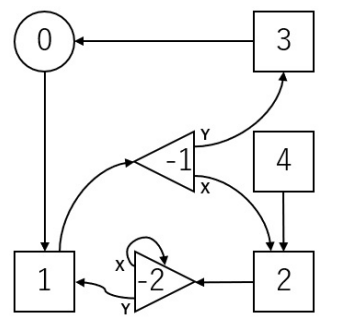
\includegraphics{4.png}

Приведенный выше рисунок показывает схему, которая описывается вызовом \texttt{answer([1, -1, -2, 0,
2], [2, -2], [3, 1])}.  Числа на рисунке~--- серийные
номера устройств. 

Используется два переключателя, поэтому $S=2$.

В начале оба переключателя $-1$ и $-2$ находятся в состоянии `X'. 

Шарик перемещается
следующим образом:

$0\rightarrow 1 \rightarrow -1 \stackrel{X}\rightarrow 2 \rightarrow -2 \stackrel{X}\rightarrow -2 \stackrel{Y}\rightarrow 1 \rightarrow -1 \stackrel{Y}\rightarrow 3 \rightarrow 0$ 

\begin{itemize}
    \item Когда шарик впервые попадает в переключатель $-1$, тот находится в
состоянии `X'. Поэтому шарик перемещается в триггер $2$. Затем состояние
переключателя $-1$ изменяется на `Y'.
\item Когда шарик попадает в переключатель $-1$ во второй раз, тот находится в
состоянии `Y'. Поэтому шарик перемещается в триггер $3$. Затем состояние
переключателя $-1$ изменяется на `X'.
\end{itemize}

Шарик впервые возвращается в источник, побывав в триггерах $1,2,1,3$. Оба
переключателя $-1$ и $-2$ находятся в состоянии `X'. Значение $P$ равно $4$.
Следовательно, эта схема удовлетворяет всем условиям.

Файл sample-01-in.txt в приложенном к задаче zip-архиве соответствует этому
примеру. Другие примеры ввода также доступны в архиве.

